\documentclass[11pt]{article}
% anderweitig wiederverwendbare Makros fuer Diss
\usepackage{amsfonts}

% allgemeine mathematische Notation
\newcommand{\ceil}[1]{\left\lceil #1\right\rceil}
\newcommand{\floor}[1]{\left\lfloor #1\right\rfloor}
\newcommand{\abs}[1]{\left| #1\right|}
\newcommand{\seq}[1]{\langle #1\rangle}
\newcommand{\norm}[1]{\left\|#1\right\|}
\newcommand{\enorm}[1]{\norm{#1}_{2}}
\newcommand{\sumnorm}[1]{\norm{#1}_{1}}
\newcommand{\maxnorm}[1]{\norm{#1}_{\infty}}
\newcommand{\xor}{\oplus}
\newcommand{\set}[1]{\left\{ #1\right\}}
\newcommand{\gilt}{:}
\newcommand{\sodass}{\,:\,}
\newcommand{\setGilt}[2]{\left\{ #1\sodass #2\right\}}
\newcommand{\Def}{:=}
\newcommand{\zvektor}[2]{\left(#1,#2\right)}
\newcommand{\vektor}[2]{\left(\begin{smallmatrix}#1\\#2\end{smallmatrix}\right)}
\newcommand{\condition}[1]{\left[#1\right]}
\newcommand{\binomial}[2]{\binom{#1}{#2}}
\newcommand{\even}{\mathrm{even}}
\newcommand{\odd}{\mathrm{odd}}
\newcommand{\mymod}{\,\bmod\,}
\newcommand{\divides}{|}

\newcommand{\blank}{\Box}
\newcommand{\cross}[2]{\langle #1,#2 \rangle}
\newcommand{\defeq}{\mathrel{:=}}
\newcommand{\hash}{\sym{@}}
\newcommand{\hD}[1][D]{^{(#1)}}
\newcommand{\hed}[1][D]{^{1/#1}}
\newcommand{\Lpal}{L_{\mathrm{pal}}}
\newcommand{\Lparity}{L_{\mathrm{parity}}}
\newcommand{\Lvv}{L_{\mathrm{vv}}}
\newcommand{\pD}[1][D]{^{[#1]}}
\newcommand{\pos}[1]{\mathbf{#1}}
\newcommand{\qs}{\mathord{\Box}}
\newcommand{\mSet}[2]{\left\{#1 \mid #2\right\}}
\newcommand{\s}{\mathord{-}}
\newcommand{\CAce}{\hbox{\mdseries\scshape CAce}}
\newcommand{\sCAce}{\s\CAce}
\newcommand{\CAcs}{\hbox{\mdseries\scshape CAcs}}
\newcommand{\sCAcs}{\s\CAcs}
\newcommand{\CAww}{\hbox{\mdseries\scshape CAww}}
\newcommand{\sCAww}{\s\CAww}
\newcommand{\sC}{\s\hbox{\scshape Chng}}
\newcommand{\sD}{\s\hbox{\scshape Diam}}
\newcommand{\sT}{\s\hbox{\scshape Time}}
\newcommand{\CA}{\hbox{\mdseries\scshape CA}}
\newcommand{\sCA}{\s\CA}
\newcommand{\ST}[1]{\langle #1\rangle}
\newcommand{\sym}[1]{\mathord{\hbox{\texttt{\upshape #1}}}}

% Typen
\newcommand{\nat}{\mathbb{N}}
\newcommand{\natnull}{\mathbb{N}_{0}}
%\newcommand{\natless}[1]{\mathbb{N}_{<#1}}
\newcommand{\natless}[1]{\mathbb{N}_{#1}}
\newcommand{\nplus}{\mathbb{N}_+}
\newcommand{\real}{\mathbb{R}}
\newcommand{\rplus}{\mathbb{R}_+}
\newcommand{\rnneg}{\mathbb{R}_*}
\newcommand{\integer}{\mathbb{Z}}
% \newcommand{\intint}[2]{\set{#1,\ldots, #2}}
\newcommand{\intint}[2]{{#1}..{#2}}
\newcommand{\realrange}[2]{\left[#1, #2\right]}
\newcommand{\realrangeo}[2]{\left(#1, #2\right)}
\newcommand{\realrangelo}[2]{\left(#1, #2\right]}
\newcommand{\realrangero}[2]{\left[#1, #2\right)}
\newcommand{\unitrange}[2]{\realrange{0}{1}}
\newcommand{\bool}{\set{0,1}}
%\newcommand{\boolean}{\mathbb{B}}
%\newcommand{\mapping}[2]{#1\rightarrow #2}
\newcommand{\mapping}[2]{{#2}^{#1}}
\newcommand{\powerset}[1]{{\cal P}\left(#1\right)}
\newcommand{\NP}{\mathbf{NP}}
\newcommand{\Bild}{\mathbf{Bild}\:}

% Typannotation
\newcommand{\withtype}[1]{\in#1}

% Wahrscheinlichkeitsrechnung
\newcommand{\prob}[1]{{\mathbf{P}}\left[#1\right]}
\newcommand{\condprob}[2]{{\mathbf{P}}\left[#1\;|\;#2\right]}
\newcommand{\condexpect}[2]{{\mathbf{E}}\left[#1\;|\;#2\right]}
\newcommand{\expect}{{\mathbf{E}}}
\newcommand{\var}{{\mathbf{Var}}}
\newcommand{\quant}[2]{\tilde{#1}_{#2}}

% asymptotische Notation
\newcommand{\whpO}[1]{\tilde{\mathrm{O}}\left( #1\right)}
\newcommand{\Oschlange}{$\tilde{\mathrm{O}}$}
\newcommand{\Ohh}[1]{\mathcal{O}\!\left( #1\right)}
\newcommand{\Oh}[1]{\mathcal{O}\!\left( #1\right)}
\newcommand{\oh}[1]{\mathrm{o}\!\left( #1\right)}
\newcommand{\Th}[1]{\Theta\!\left( #1\right)}
\newcommand{\Thsmall}[1]{\Theta( #1)}
\newcommand{\Om}[1]{\Omega\!\left( #1\right)}
\newcommand{\om}[1]{\omega\!\left( #1\right)}
\newcommand{\Oleq}{\preceq}

% local reference
\newcommand{\lref}[1]{\ref{\labelprefix:#1}}
\newcommand{\llabel}[1]{\label{\labelprefix:#1}}
\newcommand{\labelprefix}{} % later redefined using renewcommand

% Diskussion
\newcommand{\discussionsize}{\small}
\newenvironment{discussion}{\par\discussionsize}{\par}

% open issues
%\marginparwidth5cm
\marginparpush2mm
%\newcommand{\frage}[1]{\makebox[0cm]{$\bigotimes$}\marginpar{\tiny #1}}
%\newcommand{\frage}[1]{{\sf[ #1]}\marginpar{?}}
\newcommand{\frage}[1]{}

\newcommand{\mysubsubsection}[1]{\vspace{2mm}\noindent{\bf #1 }}

% punkt am ende von display math
\newcommand{\punkt}{\enspace .}

% Pseudocode Unterst\"utzung
\newenvironment{code}{\noindent%\sf%
\begin{tabbing}%
\hspace{2em}\=\hspace{2em}\=\hspace{2em}\=\hspace{2em}\=\hspace{2em}\=%
\hspace{2em}\=\hspace{2em}\=\hspace{2em}\=\hspace{2em}\=\hspace{2em}\=%
\kill}{\end{tabbing}}

% 1=pos, 2=llable, 3=caption
\newcommand{\labelcommand}{}
\newcommand{\captiontext}{}
\newsavebox{\codeparam}
\newcounter{lineNumber}
\newenvironment{disscodepos}[3]{%
\renewcommand{\labelcommand}{#2}%
\renewcommand{\captiontext}{#3}%
\sbox{\codeparam}{\parbox{\textwidth}{#3}}%
\begin{figure}[#1]\begin{center}\begin{code}\setcounter{lineNumber}{1}}{%
\end{code}\end{center}\caption{\llabel{\labelcommand}\captiontext}\end{figure}}

\newenvironment{disscode}[2]{\begin{disscodepos}{htb}{#1}{#2}}%
{\end{disscodepos}}

% code in text 
%\newcommand{\codel}[1]{{\sf #1}}
%\newcommand{\codem}[1]{\mathsf{#1}}
\newcommand{\codel}[1]{\mbox{\rm "`#1"'}}
\newcommand{\codem}[1]{\mathrm{#1}}

\newcommand{\id}{\tt}
\newcommand{\Function} {{\bf Function\ }}
\newcommand{\Procedure}{{\bf Procedure\ }}
\newcommand{\Process}{{\bf process\ }}
\newcommand{\While}    {{\bf while\ }}
\newcommand{\Repeat}   {{\bf repeat\ }}
\newcommand{\Until}    {{\bf until\ }}
\newcommand{\Loop}     {{\bf loop\ }}
\newcommand{\Exit}     {{\bf exit\ }}
\newcommand{\Goto}     {{\bf goto\ }}
\newcommand{\Do}       {{\bf do\ }}
\newcommand{\Od}       {{\bf od\ }}
\newcommand{\Dopar}       {{\bf dopar\ }}
\newcommand{\For}      {{\bf for\ }}
\newcommand{\Step}      {{\bf step\ }}
\newcommand{\Foreach}      {{\bf foreach\ }}
\newcommand{\Rof}      {{\bf rof\ }}
\newcommand{\Forall}      {{\bf forall\ }}
\newcommand{\To}       {{\bf to\ }}
\newcommand{\If}       {{\bf if\ }}
\newcommand{\Is}       {:=}
\newcommand{\Endif}    {{\bf endif\ }}
\newcommand{\Fi}       {{\bf fi\ }}
\newcommand{\Then}     {{\bf then\ }}
\newcommand{\Else}     {{\bf else\ }}
\newcommand{\Elsif}    {{\bf elsif\ }}
\newcommand{\Return}   {{\bf return\ }}
\newcommand{\Set}      {{\bf set\ }}
\newcommand{\Boolean}  {{\bf boolean\ }}
\newcommand{\Integer}  {$\integer$}
\newcommand{\True}     {{\bf true\ }}
\newcommand{\False}    {{\bf false\ }}
\newcommand{\Bitand}   {{\bf bitand\ }}
\newcommand{\Var}      {{\bf var\ }}
\newcommand{\Xor}       {{\bf\ xor\ }}
\newcommand{\Not}       {{\bf\ not\ }}
\newcommand{\Or}       {{\bf\ or\ }}
\newcommand{\Div}       {{\bf\ div\ }}
\newcommand{\Mod}       {{\bf\ mod\ }}
\newcommand{\End}       {{\bf end\ }}
\newcommand{\Endfor}       {{\bf endfor\ }}
\newcommand{\Rem}[1]   {{\bf (*~}{\rm#1}{\bf ~*)}}
% rechtsbuendiger Kommentar
%\newcommand{\RRem}[1]   {\`{$\mathbf{(*}$~ }{\rm#1}{~$\mathbf{*)}$}}
\newcommand{\RRem}[1]   {\`{\bf --\hspace{0.5mm}--~}{\rm#1}}
\newcommand{\RRemNL}[1]   {\`{\bf (*~ }{\rm#1}{\bf ~*)}%
{\tiny\arabic{lineNumber}}\stepcounter{lineNumber}}

\newcommand{\At}[1]{\left\langle#1\right\rangle}
\newcommand{\NL}{\`{\tiny\arabic{lineNumber}}\stepcounter{lineNumber}}

% Parallelverarbeitungspseudocode
\newcommand{\iProc}{i_\mathrm{PE}}

% Parameter 1=pos, 2=xsize, 3=filename, 4=llabel, 4=caption
\newcommand{\dissepslong}[5]{\begin{figure}[#1]\begin{center}%
\epsfxsize#2\leavevmode\epsfbox{#3.eps}%
\end{center}\caption{\llabel{#4}#5}\end{figure}}

\newcommand{\dissepspos}[4]{\dissepslong{#1}{#2}{\labelprefix/#3}{#3}{#4}}
\newcommand{\disseps}[3]{\dissepspos{htb}{#1}{#2}{#3}}

% Beweise
\newdimen\endofsize\endofsize=0.5em
\def\endofbeweis{~\quad\hglue\hsize minus\hsize
                 \hbox{\vrule height \endofsize width
\endofsize}\par}
% gibt es in amsmath schon
\newenvironment{myproof}{\begin{proof}}{\endofbeweis\end{proof}}
% \newcommand{\platsch}{\hglue\hsize minus\hsize}



\usepackage[utf8]{inputenc}
\usepackage{algorithmic}
\usepackage{tabularx}
\usepackage{algorithm}
\usepackage{theorem}
\usepackage{amsmath}
\usepackage{amssymb}
\usepackage{color}
\usepackage{fullpage}     
\usepackage{latexsym}
\usepackage{makeidx}
\usepackage{multicol}
\usepackage{numprint}
\usepackage{t1enc}
\usepackage{times}
\usepackage{graphicx}
\usepackage{url}
\usepackage[left=2cm,top=1.5cm,right=2cm]{geometry}
\npdecimalsign{.} % we want . not , in numbers

\definecolor{mygrey}{gray}{0.75}
\newcommand{\ie}{i.e.\ }
\newcommand{\etal}{et~al.\ }
\newcommand{\eg}{e.g.\ }
\newcommand{\Id}[1]{\ensuremath{\text{{\sf #1}}}}

\def\MdR{\ensuremath{\mathbb{R}}}
\def\MdN{\ensuremath{\mathbb{N}}}
\newcommand{\mytodo}[1]{{\color{blue}#1}}
\newcommand{\sout}[1]{{\color{mygrey}#1}}

\newcommand{\mytitle}{ {\color{red}KaDraw} v1.0 -- {\color{red}Ka}rlsruhe Graph {\color{red}Draw}ing \\ User Guide}
\begin{document}
\title{\mytitle}
\author{Henning Meyerhenke, Martin Nöllenburg and Christian Schulz\\ 
	\textit{Karlsruhe Institute of Technology (KIT)},
	\textit{Karlsruhe, Germany} \\
	\textit{Email: \{\url{meyerhenke}, \url{noellenburg}, \url{christian.schulz}\}\url{@kit.edu}} }
\date{}

\maketitle
\begin{abstract}
This paper severs as a user guide to the graph drawing framework KaDraw (Karlsruhe Graph Drawing). We give a rough overview of the techniques used within the framework and describe the user interface as well as the file formats used. 
\end{abstract}

\tableofcontents
\thispagestyle{empty}

\vfill
\pagebreak
\section{Introduction}
Drawing large networks (or graphs) with hundreds of thousands of nodes and
edges has a variety of relevant applications. One of them can be interactive visualization, which helps humans working on
graph data to gain insights about the properties of the data. If a very large high-end display is not available for such
purpose, a hierarchical approach allows the user to select an appropriate zoom level~\cite{abello-ask-06}.
Moreover, drawings of large graphs can also be used as a preprocessing step in high-performance applications~\cite{Kirmani:2013:SPG:2503210.2503280}.

One very promising class of layout algorithms in this context is based on the
\emph{stress} of a graph. Such algorithms can for instance be used for drawing graphs with fixed
distances between vertex pairs, provided \textit{a priori} in a distance matrix~\cite{gkn-gdsm-05}.
%
More recently, Gansner \etal~\cite{ghn-mmgl-13} proposed a similar model 
that includes besides the stress an additional entropy term (hence its name \emph{maxent-stress}). 
While still using shortest path distances, this model often results in more satisfactory layouts for large networks.
The optimization problem can be cast as solving Laplacian 
linear systems successively. Since each right-hand side in this succession 
depends on the previous solution, many linear systems need
to be solved until convergence.

Within KaDraw we present a novel multilevel algorithm, MulMent, to compute a graph layout with respect to maxent-stress.
%
As opposed to previous work, we do not solve the linear systems of the maxent-stress metric with a typical 
numerical solver. Instead we use a simple local iterative scheme within a multilevel approach.
To accelerate local optimization, we approximate long-range forces and parallelism.

\section{Graph Drawing Algorithms within KaDraw}
We now give a rough overview over the algorithms implemented in our framework. For details on the algorithms, we refer the interested reader to the corresponding paper~\cite{mulment}. 
A successful (meta)heuristic for graph drawing (and other optimization problems on large graphs) is the multilevel approach. We employ it for maxent-stress optimization as well.
A multilevel algorithm computes a sequence of increasingly coarse but structurally related graphs as abstractions of the original graph.
Starting from a layout of the coarsest graph, incremental refinement steps using the previous layout as a scaffold eventually produce a layout of the entire input graph, where the refinement steps are fast due to the good initial layouts. 

We briefly sketch our algorithmic 
approach: The method for creating the graph hierarchy is based on fast graph clustering with 
controllable cluster sizes~\cite{pcomplexnetworksviacluster}. 
Each cluster computed on one hierarchy level is contracted into a new supervertex for the next level.
After computing an initial layout on the coarsest hierarchy level, we improve the drawing 
on each finer level by iterating the maxent-equation to solve the maxent-stress system 
\begin{equation}
	x_{u} \gets \frac{1}{\rho_{u}} \sum_{\{u,v\}\in E} w_{uv} \left(x_{v} + d_{uv} \frac{x_{u}-x_{v}}{\Vert x_{u}-x_{v}\Vert}\right) + \frac{\alpha}{\rho_{u}} \sum_{\{u,v\}\notin E} \frac{x_{u}-x_{v}}{\Vert x_{u}-x_{v}\Vert^{2}},
\label{eq:stress-entropy-iter}
\end{equation}
where $\rho_{u}=\sum_{\{u,v\}\in E}w_{uv}$ and appropriately chosen weights and distances are used. 
Additionally, this process exploits
the hierarchy and draws vertices that are densely connected with each other (\ie which are in the same cluster) close to each other.
Note that the local optimization algorithm presented above has a theoretical running time of $\mathcal{O}(n^2)$ per iteration.
To speed this up, our algorithm uses approximations for the distances in the entropy term in Eq.~(\ref{eq:stress-entropy-iter}).
We do this by taking the cluster structure computed during coarsening into account, \ie we use graphs and coordinates multiple levels beneath the current level under consideration to approximate the second summation in Eq.~(\ref{eq:stress-entropy-iter}). For more details, we refer the reader to the paper~\cite{mulment}.




\paragraph{Shared-memory Parallelization.}
%
Local optimization algorithms use shared-memory parallelism (OpenMP).
An iteration of the local optimizer works as follows: Since new coordinates of the vertices in the same iteration can be computed independently, we use multiple threads to do so. 
Parallelism is also used analogously when working on different levels for the distance approximations
in the entropy term.



\vfill
\pagebreak
\,
\pagebreak
\section{Graph Format}
\label{ss:graphformat}
\subsection{Input File Format}
The graph format used by our partitioning programs is the same as used by Metis \cite{karypis1998fast}, Chaco \cite{chaco} and the graph format that has been used during the 10th DIMACS Implementation Challenge on Graph Clustering and Partitioning. 
The input graph has to be undirected, withoud self-loops and without parallel edges.

To give a description of the graph format, we follow the description of the Metis 4.0 user guide very closely. A graph $G=(V,E)$ with $n$ vertices and $m$ edges is stored in a plain text file that contains $n+1$ lines (excluding comment lines). The first line contains information about the size and the type of the graph, while the remaining $n$ lines contain information for each vertex of $G$. Any line that starts with \% is a comment line and is skipped.

The first line in the file contains either two integers, $n$ $m$, or three integers, $n$ $m$ $f$. The first two integers are the number of vertices $n$ and the number of undirected edges of the graph, respectively. Note that in determining the number of edges $m$, an edge between any pair of vertices $v$ and $u$ is counted \emph{only once} and not twice, \ie we do not count the edge $(v,u)$ from $(u,v)$ separately. The third integer $f$ is used to specify whether or not the graph has weights associated with its vertices, its edges or both. If the graph is unweighted then this parameter can be omitted. It should be set to $1$ if the graph has edge weights, 10 if the graph has node weights and 11 if the graph has edge and node weights.

The remaining $n$ lines of the file store information about the actual structure of the graph. In particular, the $i$th line (again excluding comment lines) contains information about the $i$th vertex. Depending on the value of $f$, the information stored in each line is somewhat different. In the most general form (when $f=11$, \ie we have node and edge weights) each line has the following structure:
\begin{center}
       $c\, v_1\, w_1\, v_2\, w_2 \ldots v_k\, w_k$ 
\end{center}
where $c$ is the vertex weight associated with this vertex, $v_1, \ldots, v_k$ are the vertices adjacent to this vertex, and $w_1, \ldots, w_k$ are the weights of the edges. Note that the vertices are numbered starting from 1 (not from 0). Furthermore, the vertex-weights must be integers greater or equal to 0, whereas the edge-weights must be strictly greater than 0.

\begin{figure}[h!]
\begin{center}
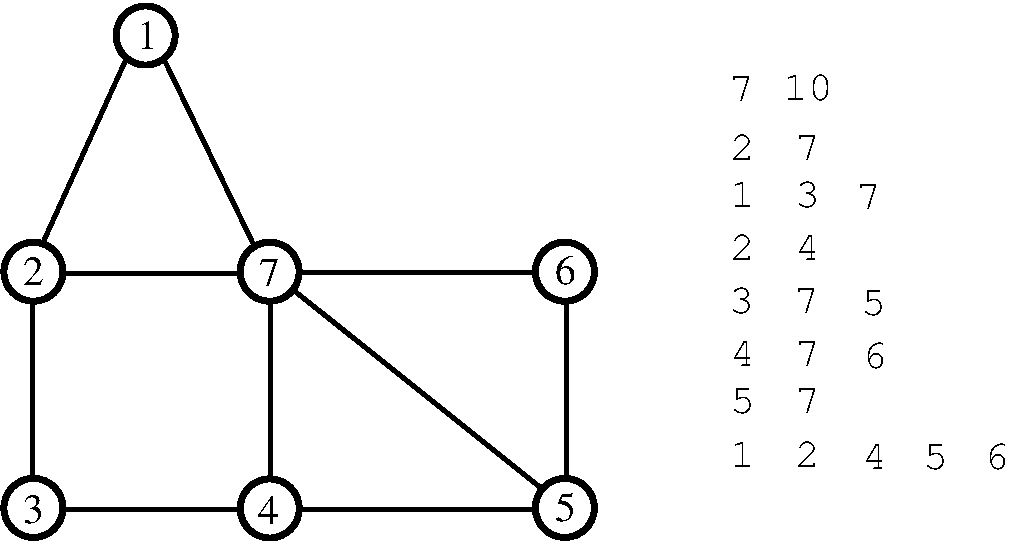
\includegraphics[width=.8\textwidth]{example_graph.pdf}
\end{center}

\caption{An example graph and its representation in the graph format. The IDs of the vertices are drawn within the cycle, the vertex weight is shown next to the circle ({\color{red}red}) and the edge weight is plotted next to the edge ({\color{blue}blue}).}
\label{fig:example}
\end{figure}
\subsection{Output File Formats}
\subsubsection{Coordinate File}
The output format of coordinates is basically a text file. 
This file contains $n$ lines. 
In each line the 2D-coordinate of the corresponding vertex is given, \ie line $i$ contains the coordinate of vertex $i$.
\subsubsection{PDF/PNG files}
If the output is a node separator then the same format as used for a partition is used. However, in this case the nodes of the separator get the block ID $k$ where as the other nodes maintain their original block id. 
\subsection{Troubleshooting}
KaDraw should not crash! If KaDraw crashes it is mostly due to the following reasons: the provided graph contains self-loops or parallel edges, there exists a forward edge but the backward edge is missing or the forward and backward edges have different weights, or the number of vertices or edges specified does not match the number of vertices or edges provided in the file.
Please use the \emph{graphcheck} tool provided in our graph partitioning package to verify whether your graph has the right input format. If our graphcheck tool tells you that the graph that you provided has the correct format and KaDraw crashes anyway, please write us an email.

\vfill
\pagebreak
\section{User Interface}
KaDraw contains the following programs: kadraw, graphchecker, evaluator, draw\_from\_coordinates. To compile these programs you need to have Argtable, g++, OpenMP and scons installed (we use argtable-2.10, g++-4.8.0 and scons-1.2). Once you have that you can execute \emph{compile.sh} in the main folder of the release. When the process is finished the binaries can be found in the folder \emph{deploy}. We now explain the parameters of each of the programs briefly.
\subsection{KaDraw}
\paragraph*{Description:} This is the multilevel graph drawing program. 
\paragraph*{Usage:\\} 

\begin{tabular}{ll}
kadraw &   [-{}-help] FILE [-{}-seed=<int>] [-{}-preconfiguration=VARIANT]  \\
& [-{}-burn\_coordinates\_to\_disk] [-{}-burn\_image\_to\_disk] [-{}-output\_filename=<string>] \\ 
& [-{}-image\_scale=<double>] [-{}-num\_threads=<int>] [-{}-export\_type=TYPE] [-{}-linewidth=<double>] \\ 
& [-{}-compute\_FSM] [-{}-compute\_MEnt]

\end{tabular}
                          
\subsection*{Options:\\}

\begin{tabularx}{\textwidth}{lX}
  FILE                          & Path to graph file to draw.\\
  --help                        & Print help. \\
  --seed=<int>                  & Seed to use for the PRNG.\\
  --preconfiguration=VARIANT    & Use a preconfiguration. (Default: fast) [strong|eco|fast].\\
  --burn\_coordinates\_to\_disk & Save the coordinates in a file.\\
  --burn\_image\_to\_disk       & Save the image in a file.\\
  --export\_type=TYPE           & Specify export type. [pdf|png]\\
  --output\_filename=<string>   & Output filename of the png/pdf file.\\
  --image\_scale=<double>       & Set image scale manually.\\
  --num\_threads=<int>          & Set the number of OMP threads (default: maximum available number used).\\
  --linewidth=<double>          & Line width to use for drawing.\\
  --compute\_FSM                & Enable computation of Full Stress Measure.\\
  --compute\_MEnt               & Enable computation of MaxEnt-stress at a penalty level of 0.008.\\
\end{tabularx}
\vfill
\pagebreak
\subsection{Evaluator}
\paragraph*{Description:} This program takes a graph and its coordinates and computes various performance metrics.
\paragraph*{Usage:\\} 

\begin{tabular}{ll}
evaluator &   [-{}-help] FILE [-{}-seed=<int>] [-{}-print\_final\_distances]  \\
& [-{}-compute\_FSM] [-{}-compute\_MEnt] [--coordfilename=<string>]

\end{tabular}
                          
\subsection*{Options:\\}

\begin{tabularx}{\textwidth}{lX}
  FILE                          & Path to graph file to evaluate.\\
  --help                        & Print help. \\
  --print\_final\_distances     & Print the final distances. \\
  --compute\_FSM                & Enable computation of Full Stress Measure.\\
  --compute\_MEnt               & Enable computation of MaxEnt-stress at a penalty level of 0.008.\\
  --coordfilename=<string>      & Filename of input coordinates to evaluate. \\
\end{tabularx}
\subsection{DrawGraphFromCoordinates}
\paragraph*{Description:} This program takes a graph and its coordinates and outputs a pdf/png file containing the drawn graph.
\paragraph*{Usage:\\} 

\begin{tabular}{ll}
 draw\_from\_coordinates&   [-{}-help] FILE [-{}-export\_type=TYPE]  \\
& [--coordfilename=<string>] [--output\_filename=<string>]



\end{tabular}
                          
\subsection*{Options:\\}

\begin{tabularx}{\textwidth}{lX}
  FILE                          & Path to graph file to draw.\\
  --help                        & Print help. \\
  --export\_type=TYPE           & Specify export type. [pdf|png]\\
  --output\_filename=<string>   & Output filename of the png/pdf file. \\
  --coordfilename=<string>      & Filename of input coordinates to evaluate. \\
\end{tabularx}

\vfill
\pagebreak
\vfill
\pagebreak
\subsection{Graph Format Checker}
\paragraph*{Description:} This program checks if the graph specified in a given file is valid. 
\paragraph*{Usage:\\} 
\begin{tabular}{ll}
graphchecker & file
\end{tabular}
\subsection*{Options:\\} 
\begin{tabularx}{\textwidth}{lX}
  file                       & Path to the graph file. \\
\end{tabularx}

\vfill
\pagebreak
\vfill
\pagebreak
\bibliographystyle{plain}
%\bibliography{phdthesiscs,masterReferences,references,Bibliography}
\begin{thebibliography}{1}

\bibitem{abello-ask-06}
J.~Abello, F.~van Ham, and Neeraj K.
\newblock Ask-graphview: A large scale graph visualization system.
\newblock {\em {IEEE} Trans. Visualization and Computer Graphics},
  12(5):669--676, 2006.

\bibitem{ghn-mmgl-13}
E.~R. Gansner, Y.~Hu, and S.~C. North.
\newblock A maxent-stress model for graph layout.
\newblock {\em {IEEE} Trans. Visualization and Computer Graphics},
  19(6):927--940, 2013.

\bibitem{gkn-gdsm-05}
E.~R. Gansner, Y.~Koren, and S.~North.
\newblock Graph drawing by stress majorization.
\newblock In {\em Graph Drawing (GD'04)}, volume 3383 of {\em LNCS}, pages
  239--250. Springer, 2005.

\bibitem{chaco}
B.~Hendrickson.
\newblock {Chaco: Software for Partitioning Graphs}.
\newblock {\url{http://www.cs.sandia.gov/~bahendr/chaco.html}}.

\bibitem{karypis1998fast}
G.~Karypis and V.~Kumar.
\newblock {A Fast and High Quality Multilevel Scheme for Partitioning Irregular
  Graphs}.
\newblock {\em SIAM Journal on Scientific Computing}, 20(1):359--392, 1998.

\bibitem{Kirmani:2013:SPG:2503210.2503280}
S.~Kirmani and P.~Raghavan.
\newblock Scalable parallel graph partitioning.
\newblock In {\em Proceedings of the International Conference on High
  Performance Computing, Networking, Storage and Analysis}, SC '13, pages
  51:1--51:10, New York, NY, USA, 2013. ACM.

\bibitem{mulment}
H.~Meyerhenke, M.~Nöllenburg, and C.~Schulz.
\newblock Drawing large graphs by multilevel maxent-stress optimization.
\newblock Technical report, 2015.

\bibitem{pcomplexnetworksviacluster}
H.~Meyerhenke, P.~Sanders, and C.~Schulz.
\newblock {Partitioning Complex Networks via Size-constrained Clustering}.
\newblock In {\em 13th Int. Symp. on Exp. Algorithms}, LNCS. Springer, 2014.

\end{thebibliography}
\end{document}


